\section{Reverse-Mode Automatic Differentiation}
\frame{\tableofcontents[currentsection]}

\begin{frame}
\frametitle{Example Function and Expression Graph}
\[f(x_1, x_2, x_3) = \sin(x_1) + \cos(x_2) \cdot x_3 - \log(x_3)\]

\pause%

% Original expression graph
\begin{figure}[t]
\centering
\scalebox{0.9}{%

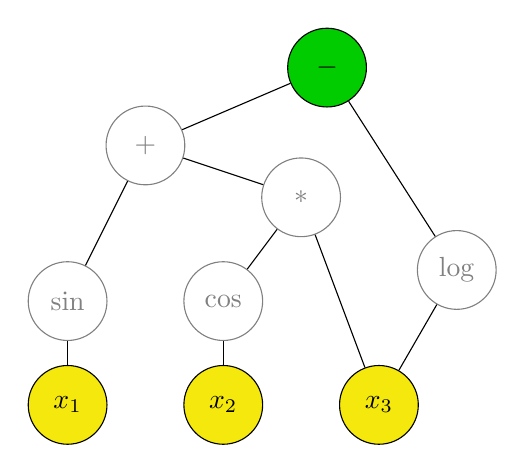
\begin{tikzpicture}[x=0.75pt,y=0.75pt,yscale=-0.5,xscale=0.5]

    \draw (150,350) node [align=center, minimum size=1cm, draw, circle, fill=black!5!yellow] (x1)  {$x_1$};
    \draw (300,350) node [align=center, minimum size=1cm, draw, circle, fill=black!5!yellow] (x2)  {$x_2$};
    \draw (450,350) node [align=center, minimum size=1cm, draw, circle, fill=black!5!yellow] (x3)  {$x_3$};
    \draw (150,250) node [align=center, minimum size=1cm, draw, circle, color=gray] (sin) {$\sin$};
    \draw (300,250) node [align=center, minimum size=1cm, draw, circle, color=gray] (cos) {$\cos$};
    \draw (525,220) node [align=center, minimum size=1cm, draw, circle, color=gray] (log) {$\log$};
    \draw (225,100) node [align=center, minimum size=1cm, draw, circle, color=gray] (add) {$+$};
    \draw (375,150) node [align=center, minimum size=1cm, draw, circle, color=gray] (mul) {$*$};
    \draw (400,25)  node [align=center, minimum size=1cm, draw, circle, fill=black!20!green] (sub) {$-$};
    \draw (x1) -- (sin);
    \draw (x2) -- (cos);
    \draw (x3) -- (mul);
    \draw (x3) -- (log);
    \draw (sin) -- (add);
    \draw (cos) -- (mul);
    \draw (mul) -- (add);
    \draw (add) -- (sub);
    \draw (log) -- (sub);

\end{tikzpicture}
} % end scalebox

\end{figure}
\end{frame}

% Explain what we modify to get from expr graph -> tree
\begin{frame}
\frametitle{Expression Tree Conversion}
\begin{itemize}
\item $x_i$ can be referenced by multiple nodes.
    \begin{itemize}
        \item e.g. $x_3$ is referenced by the \code{*} and \code{log} nodes.
    \end{itemize}

\item Convert expression graph into an expression tree.
    \begin{itemize}
        \item Replace all nodes with multiple parents as separate nodes
            that reference back to the actual variables.
    \end{itemize}

\item Mathematically,
\begin{align}
    f(x_1, x_2, x_3) &= \tilde{f}(g(x_1, x_2, x_3)) \label{eq:f-tree-example} \\
    \tilde{f}(w_1, w_2, w_3, w_4) &= \sin(w_1) + \cos(w_2) \cdot w_3 - \log(w_4) \nonumber \\
    g(x_1, x_2, x_3) &= (x_1, x_2, x_3, x_3) \nonumber
\end{align}

\end{itemize}
\end{frame}

% Expression tree
\begin{frame}
\frametitle{Expression Tree Conversion}

\begin{figure}[t]
\centering

\scalebox{0.9}{%

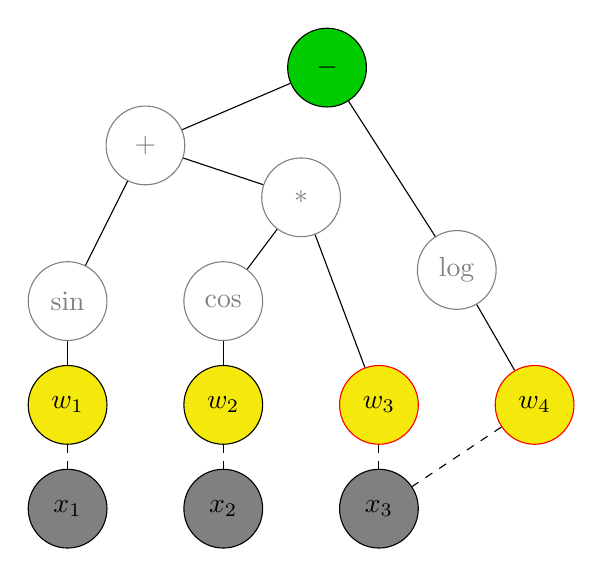
\begin{tikzpicture}[x=0.75pt,y=0.75pt,yscale=-0.5,xscale=0.5]

    \draw (150,450) node [align=center, minimum size=1cm, draw, circle, fill=gray] (x1)  {$x_1$};
    \draw (300,450) node [align=center, minimum size=1cm, draw, circle, fill=gray] (x2)  {$x_2$};
    \draw (450,450) node [align=center, minimum size=1cm, draw, circle, fill=gray] (x3)  {$x_3$};
    \draw (150,350) node [align=center, minimum size=1cm, draw, circle, fill=black!5!yellow] (w1)  {$w_1$};
    \draw (300,350) node [align=center, minimum size=1cm, draw, circle, fill=black!5!yellow] (w2)  {$w_2$};
    \draw (450,350) node [align=center, minimum size=1cm, draw=red, circle, fill=black!5!yellow] (w3)  {$w_3$};
    \draw (600,350) node [align=center, minimum size=1cm, draw=red, circle, fill=black!5!yellow] (w4)  {$w_4$};
    \draw (150,250) node [align=center, minimum size=1cm, draw, circle, color=gray] (sin) {$\sin$};
    \draw (300,250) node [align=center, minimum size=1cm, draw, circle, color=gray] (cos) {$\cos$};
    \draw (525,220) node [align=center, minimum size=1cm, draw, circle, color=gray] (log) {$\log$};
    \draw (225,100) node [align=center, minimum size=1cm, draw, circle, color=gray] (add) {$+$};
    \draw (375,150) node [align=center, minimum size=1cm, draw, circle, color=gray] (mul) {$*$};
    \draw (400,25)  node [align=center, minimum size=1cm, draw, circle, fill=black!20!green] (sub) {$-$};
    \draw [dashed] (w1) -- (x1);
    \draw [dashed] (w2) -- (x2);
    \draw [dashed] (w3) -- (x3);
    \draw [dashed] (w4) -- (x3);
    \draw (w1) -- (sin);
    \draw (w2) -- (cos);
    \draw (w3) -- (mul);
    \draw (w4) -- (log);
    \draw (sin) -- (add);
    \draw (cos) -- (mul);
    \draw (mul) -- (add);
    \draw (add) -- (sub);
    \draw (log) -- (sub);

\end{tikzpicture}

} % end scalebox

\end{figure}
\end{frame}

% Explain why we do conversion
\begin{frame}
\frametitle{Expression Tree Conversion}

\begin{itemize}

\item{Why do we need this conversion?}
    \begin{itemize}
        \item All nodes except \code{$x_i$} have exactly one parent.
        \item Leads to cleaner implementation.
        \item Better to treat $x_i$ as \emph{containers} for
            initial values and their \textbf{adjoints}, $\frac{\partial f}{\partial x_i}$,
            instead of nodes of the graph.
    \end{itemize}

\end{itemize}
\end{frame}

% Introduce AD algorithm
\begin{frame}
\frametitle{Reverse-Mode AD Algorithm}
\begin{itemize}

\item Assume for the moment that $f: \R^n \to \R$.

\item Reverse-mode algorithm consists of two passes of the expression tree:
    \begin{itemize}
        \item \emph{forward}-evaluation (not to be confused with forward-mode AD)
        \item \emph{backward}-evaluation
    \end{itemize}

\end{itemize}
\end{frame}

% Explain forward-evaluation
\begin{frame}
\frametitle{Forward-Evaluation}
\begin{itemize}

\item Compute expression in the usual fashion.
    \begin{itemize}
        \item Start at the root.
        \item Recursively forward-evaluate left to right all its children.
        \item Compute current node operation using children results.
            \begin{itemize}
                \item e.g.\ for \code{sin} node, $x_1 \to w_1 \to \sin(w_1)$
            \end{itemize}
    \end{itemize}

\end{itemize}
\end{frame}

% Continue explaining forward-eval with picture
\begin{frame}
\frametitle{Forward-Evaluation}
\begin{figure}[t]
\centering

\scalebox{0.9}{%

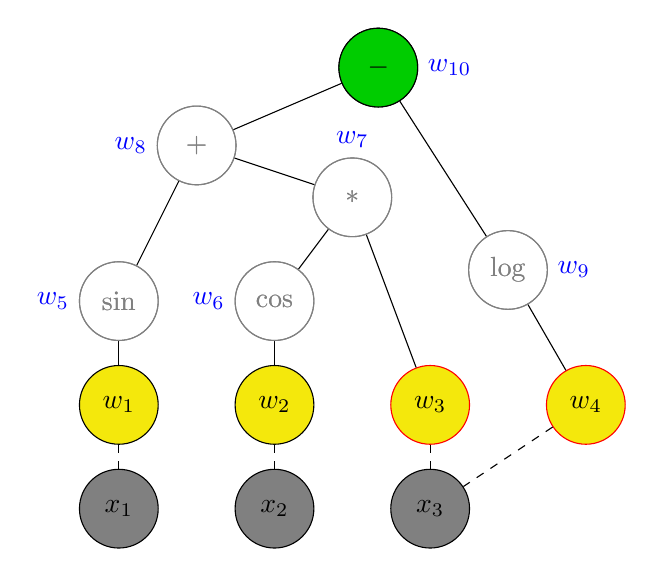
\begin{tikzpicture}[x=0.75pt,y=0.75pt,yscale=-0.5,xscale=0.5]

    \draw (150,450) node [align=center, minimum size=1cm, draw, circle, fill=gray] (x1)  {$x_1$};
    \draw (300,450) node [align=center, minimum size=1cm, draw, circle, fill=gray] (x2)  {$x_2$};
    \draw (450,450) node [align=center, minimum size=1cm, draw, circle, fill=gray] (x3)  {$x_3$};
    \draw (150,350) node [align=center, minimum size=1cm, draw, circle, fill=black!5!yellow] (w1)  {$w_1$};
    \draw (300,350) node [align=center, minimum size=1cm, draw, circle, fill=black!5!yellow] (w2)  {$w_2$};
    \draw (450,350) node [align=center, minimum size=1cm, draw=red, circle, fill=black!5!yellow] (w3)  {$w_3$};
    \draw (600,350) node [align=center, minimum size=1cm, draw=red, circle, fill=black!5!yellow] (w4)  {$w_4$};
    \draw (150,250) node [align=center, minimum size=1cm, draw, circle, color=gray] (sin) {$\sin$};
    \draw (300,250) node [align=center, minimum size=1cm, draw, circle, color=gray] (cos) {$\cos$};
    \draw (525,220) node [align=center, minimum size=1cm, draw, circle, color=gray] (log) {$\log$};
    \draw (225,100) node [align=center, minimum size=1cm, draw, circle, color=gray] (add) {$+$};
    \draw (375,150) node [align=center, minimum size=1cm, draw, circle, color=gray] (mul) {$*$};
    \draw (400,25)  node [align=center, minimum size=1cm, draw, circle, fill=black!20!green] (sub) {$-$};
    \draw [dashed] (w1) -- (x1);
    \draw [dashed] (w2) -- (x2);
    \draw [dashed] (w3) -- (x3);
    \draw [dashed] (w4) -- (x3);
    \draw (w1) -- (sin);
    \draw (w2) -- (cos);
    \draw (w3) -- (mul);
    \draw (w4) -- (log);
    \draw (sin) -- (add);
    \draw (cos) -- (mul);
    \draw (mul) -- (add);
    \draw (add) -- (sub);
    \draw (log) -- (sub);

    \pause%
    \draw (150,250) node [align=center, minimum size=1cm,
                          draw, circle, color=gray,
                          label={[blue]left:$w_5$}] (sin) {$\sin$};
    \pause%
    \draw (300,250) node [align=center, minimum size=1cm,
                          draw, circle, color=gray,
                          label={[blue]left:$w_6$}] (cos) {$\cos$};
    \pause%
    \draw (375,150) node [align=center, minimum size=1cm,
                          draw, circle, color=gray,
                          label={[blue]90:$w_7$}] (mul) {$*$};

    \pause%
    \draw (225,100) node [align=center, minimum size=1cm,
                          draw, circle, color=gray,
                          label={[blue]left:$w_8$}] (add) {$+$};

    \pause%
    \draw (525,220) node [align=center, minimum size=1cm,
                          draw, circle, color=gray,
                          label={[blue]right:$w_9$}] (log) {$\log$};
    \pause%
    \draw (400,25)  node [align=center, minimum size=1cm,
                          draw, circle, fill=black!20!green,
                          label={[blue]right:$w_{10}$}] (sub) {$-$};

\end{tikzpicture}

} % end scalebox

\end{figure}
\end{frame}

% Explain back-eval algorithm
\begin{frame}
\frametitle{Backward-Evaluation}
\begin{itemize}

\item Current node receives its adjoint from its parent.

\item This adjoint is also referred to as \emph{seed}.

\item Hence, root will receive seed = 1 from the caller.

\item Current node computes seeds for all its children and
    recursively backward-evaluates from \emph{right-to-left}.

\end{itemize}
\end{frame}

% Explain how to compute next seeds
\begin{frame}
\frametitle{Backward-Evaluation: Computing Next Seed}
\begin{itemize}

\item Next seed is computed by a simple chain-rule.
\item Let the current node be $w \in \R^{p \times q}$ and $v \in \R^{m \times n}$ one of its children.
\item The seed for $v$ is given by
\begin{align}
    \frac{\partial f}{\partial v_{ij}} &=
        \sum\limits_{k=1}^p \sum\limits_{l=1}^q
        \frac{\partial f}{\partial w_{kl}} \frac{\partial w_{kl}}{\partial v_{ij}}
    \label{eq:next-adj}
\end{align}
\item Since we are working with an expression tree,
    $f$ only depends on $v$ through $w$, hence this is the full adjoint.

\end{itemize}
\end{frame}

\begin{frame}
\frametitle{Backward-Evaluation: Computing Next Seed}
\begin{itemize}

\item Nodes with reference to containers must increment
    the adjoints in the containers with their seed.
    \begin{itemize}
        \item e.g.\ $w_3$ and $w_4$ increments the adjoint in $x_3$ with their seeds.
    \end{itemize}

\item Why? Chain-rule, once again.

\item Let $w_1, \ldots, w_k$ denote all variables with a reference to $x$.
    For simplicity assume they are all scalars (easily generalizable).
    Then,
    \begin{align*}
        \frac{\partial f}{\partial x}
        &=  \sum\limits_{i=1}^k
            \frac{\partial f}{\partial w_{i}} \frac{\partial w_{i}}{\partial x}
        =   \sum\limits_{i=1}^k
            \frac{\partial f}{\partial w_{i}}
    \end{align*}

\item Accumulated adjoints for $x_1, x_2, x_3$ is the gradient of $f$.

\end{itemize}
\end{frame}

% Back-eval with picture
\begin{frame}
\frametitle{Backward-Evaluation}
\begin{figure}[t]
\centering

\scalebox{0.9}{%

\begin{tikzpicture}[x=0.75pt,y=0.75pt,yscale=-0.5,xscale=0.5]

    \draw (150,450) node [align=center, minimum size=1cm, draw, circle, fill=gray] (x1)  {$x_1$};
    \draw (300,450) node [align=center, minimum size=1cm, draw, circle, fill=gray] (x2)  {$x_2$};
    \draw (450,450) node [align=center, minimum size=1cm, draw, circle, fill=gray] (x3)  {$x_3$};
    \draw (150,350) node [align=center, minimum size=1cm, draw, circle, fill=black!5!yellow] (w1)  {$w_1$};
    \draw (300,350) node [align=center, minimum size=1cm, draw, circle, fill=black!5!yellow] (w2)  {$w_2$};
    \draw (450,350) node [align=center, minimum size=1cm, draw=red, circle, fill=black!5!yellow] (w3)  {$w_3$};
    \draw (600,350) node [align=center, minimum size=1cm, draw=red, circle, fill=black!5!yellow] (w4)  {$w_4$};
    \draw (150,250) node [align=center, minimum size=1cm, draw, circle, color=gray] (sin) {$\sin$};
    \draw (300,250) node [align=center, minimum size=1cm, draw, circle, color=gray] (cos) {$\cos$};
    \draw (525,220) node [align=center, minimum size=1cm, draw, circle, color=gray] (log) {$\log$};
    \draw (225,100) node [align=center, minimum size=1cm, draw, circle, color=gray] (add) {$+$};
    \draw (375,150) node [align=center, minimum size=1cm, draw, circle, color=gray] (mul) {$*$};
    \draw (400,25)  node [align=center, minimum size=1cm, draw, circle, fill=black!20!green] (sub) {$-$};
    \draw [dashed] (w1) -- (x1);
    \draw [dashed] (w2) -- (x2);
    \draw [dashed] (w3) -- (x3);
    \draw [dashed] (w4) -- (x3);
    \draw (w1) -- (sin);
    \draw (w2) -- (cos);
    \draw (w3) -- (mul);
    \draw (w4) -- (log);
    \draw (sin) -- (add);
    \draw (cos) -- (mul);
    \draw (mul) -- (add);
    \draw (add) -- (sub);
    \draw (log) -- (sub);

    % Leftover labelling from forward-evaluation
    \draw (150,250) node [align=center, minimum size=1cm,
                          draw, circle, color=gray,
                          label={[blue]left:$w_5$}] (sin) {$\sin$};
    \draw (300,250) node [align=center, minimum size=1cm,
                          draw, circle, color=gray,
                          label={[blue]left:$w_6$}] (cos) {$\cos$};
    \draw (375,150) node [align=center, minimum size=1cm,
                          draw, circle, color=gray,
                          label={[blue]90:$w_7$}] (mul) {$*$};
    \draw (225,100) node [align=center, minimum size=1cm,
                          draw, circle, color=gray,
                          label={[blue]left:$w_8$}] (add) {$+$};
    \draw (525,220) node [align=center, minimum size=1cm,
                          draw, circle, color=gray,
                          label={[blue]right:$w_9$}] (log) {$\log$};
    \draw (400,25)  node [align=center, minimum size=1cm,
                          draw, circle, fill=black!20!green,
                          label={[blue]right:$w_{10}$}] (sub) {$-$};

    \pause%
    \draw [red] (sub) -- (log) node[midway, label={[red]right:$-1$}];

    \pause%
    \draw [red] (log) -- (w4) node[midway, label={[red]right:$\frac{-1}{w_4}$}];

    \pause%
    \draw [red, dashed] (w4) -- (x3) node[midway, label={[red]280:$\frac{-1}{w_4}$}];

    \pause%
    \draw [red] (sub) -- (add) node[midway, label={[red]100:$1$}];

    \pause%
    \draw [red] (add) -- (mul) node[midway, label={[red]90:$1$}];

    \pause%
    \draw [red] (mul) -- (w3) node[midway, label={[red]-20:$w_6$}];

    \pause%
    \draw [red, dashed] (w3) -- (x3) node[midway, label={[red]left:$w_6$}];

    \pause%
    \draw [red] (mul) -- (cos) node[midway, label={[red]100:$w_3$}];

    \pause%
    \draw [red] (cos) -- (w2) node[midway, label={[red]left:\scriptsize $-w_3\sin(w_2)$}];

    \pause%
    \draw [red, dashed] (w2) -- (x2) node[midway, label={[red]left:\scriptsize $-w_3\sin(w_2)$}];

    \pause%
    \draw [red] (add) -- (sin) node[midway, label={[red]100:$1$}];

    \pause%
    \draw [red] (sin) -- (w1) node[midway, label={[red]left:\scriptsize $\cos(w_1)$}];

    \pause%
    \draw [red, dashed] (w1) -- (x1) node[midway, label={[red]left:\scriptsize $\cos(w_1)$}];

\end{tikzpicture}

} % end scalebox
\end{figure}
\end{frame}

\begin{frame}{Backward-Evaluation}
\begin{itemize}
    \item Sanity check:
    \begin{align*}
        f(x_1, x_2, x_3) &= \sin(x_1) + \cos(x_2) \cdot x_3 - \log(x_3) \\
        \nabla f &= \paren{\cos(x_1), -x_3\sin(x_2), \cos(x_2)-x_3^{-1}}
    \end{align*}
\end{itemize} 
\end{frame}

\begin{frame}{Remarks}
\begin{itemize}
    \item Much harder to implement (memory management is tricky).
    \item Fast for $f:\R^n \to \R^m$ where $n \gg m$ ($O(m)$ sweeps of computation graph).
    \item Useful when we need to compute gradient (of a scalar function).
    \item Example code:
    \begin{itemize}
        \item \code{rv\_ad}
        \item \code{for\_each}
        \item \code{if\_else}
    \end{itemize}
\end{itemize} 
\end{frame}